%!TEX program = xelatex

\documentclass[a4paper,11pt]{article}
%\usepackage[cp1250]{inputenc} %Czech and Slovak symbols
%\usepackage{a4wide}
\usepackage{setspace}
\usepackage{graphicx}
\usepackage{amsmath, amsthm, amssymb} %better typesetting of mathematical expressions, theorems, additional symbols
\usepackage{booktabs}%fixltx2e}
\usepackage[flushleft]{threeparttable}
\usepackage{tabularx}
\usepackage[capposition=top]{floatrow}
\usepackage{caption}
\captionsetup[measuredfigure]{labelformat=empty}
\usepackage{bm}
\usepackage{subcaption}
\usepackage{epstopdf} % not supported by xelatex
\usepackage{fullpage}
\usepackage{enumerate}
\usepackage{setspace}
\usepackage{authblk}
%\usepackage{fontspec}
\usepackage{lscape}
\usepackage[round]{natbib} %standard package for bibliography
\usepackage{multirow}
\usepackage[figuresleft]{rotating}
\usepackage[dvipsnames]{xcolor}
\usepackage{colortbl}
\usepackage{geometry}
\usepackage{hyperref} %hyperlink support
\hypersetup{pdfstartview={XYZ null null 1.00},bookmarksnumbered, hypertexnames=false, colorlinks=true, linkcolor=BrickRed, citecolor=MidnightBlue, urlcolor=MidnightBlue} %zoom: default screen; numbers for bookmarks

%
%
%\usepackage{parskip}
\usepackage[nolist]{acronym}
\usepackage{longtable}
\acrodef{bma}[BMA]{Bayesian Model Averaging}
\acrodef{bic}[BIC]{Bayesian Information Criterion}
\acrodef{cbf}[CBF]{Conditional Bayes Factor}
\acrodefplural{cbf}[CBFs]{Conditional Bayes Factors}
\acrodef{cswd}[CSWD]{Credit Suisse Wealth Databook}
\acrodef{gfdd}[GFDD]{Global Financial Development Database}
\acrodef{pip}[PIP]{Posterior Inclusion Probability}
\acrodefplural{pip}[PIPs]{Posterior Inclusion Probabilities}
\acrodef{fdi}[FDI]{Foreign Direct Investment}
\acrodefplural{fdi}[FDIs]{Foreign Direct Investments}
\acrodef{gdp}[GDP]{Gross Domestic Product}
\acrodef{uip}[UIP]{Unit Information Prior}
\acrodef{wb}[WB]{World Bank}
\acrodef{oecd}[OECD]{Organisation for Co-operation and Development}
\acrodef{ivbma}[IVBMA]{Instrumental Variable Bayesian Model Averaging}
\acrodef{wid}[WID]{World Inequality Database}
\acrodef{hbs}[HBS]{Household Balance Sheet}
\acrodef{uk}[UK]{United Kingdom}
\acrodef{us}[US]{United States}
\acrodef{efw}[EFW]{Economic Freedom of the World}
\acrodef{pmp}[PMP]{Posterior Model Probability}

%
%
\setcounter{page}{1}

\setlength\parindent{34pt}
\onehalfspacing
\title{Finance and Wealth Inequality\thanks{We thank two anonymous referees, Joshua Aizenman, Trinil Arimurti, Nauro Campos, Alex Cukierman, Michael Koetter, Lubos Pastor, Fabien Rondeau and Dimitrios Tsomocos for helpful discussions and seminar participants at the Annual International Conference on Macroeconomic Analysis and International Finance, European Public Choice Annual Conference, Financial Engineering and Banking Society Annual Conference, Multinational Finance Society Annual Conference, Charles University, Leibniz Institute for East and Southeast European Studies and University of Economics, Prague for helpful comments. Horvath acknowledges support from the Czech Science Foundation No. 19-15650S. Mares acknowledges the hospitality of Columbia University, where he stayed as visiting researcher in January-April 2018 thanks to the support by the H2020-MSCA-RISE project GEMCLIME-2020 GA No. 681228, and support from Grant Agency of Charles University No. 768217. Horvath acknowledges the hospitality of Leibniz Institute for East and Southeast European Studies, where he stayed as visiting researcher in January-February 2018. Horvath and Mares acknowledge support from Charles University Research Centre program No. UNCE/HUM/035. Hasan acknowledges the financial support from the Australian Research Council via Discovery Grant DP170101413 for this research. Online Appendix is available at https://ies.fsv.cuni.cz/en/staff/horvath. The views are not necessarily of Bank of Finland.}}


\author[a,b,c]{Iftekhar Hasan}
\author[d,e]{Roman Horvath}
\author[d]{Jan Mares\footnote{\footnotesize Corresponding author's address: IES FSV UK, Opletalova 26, 110 00, Praha 1; \textbf{e-mail:janxmares@gmail.com}}}
\affil[a]{Fordham University}
\affil[b]{Bank of Finland}
\affil[c]{University of Sydney}
\affil[d]{Charles University, Prague}
\affil[e]{University of Ss. Cyril and Methodius in Trnava}


%\renewcommand\Authands{ and }
\date{\today}
%\bibliographystyle{stylebib}
\begin{document}

\clubpenalty 9999 %no orphants (typographic properties)
\widowpenalty 9999 %no widows (typographic properties)
\def\sym#1{\ifmmode^{#1}\else\(^{#1}\)\fi} %shortcut for Stata tables

\maketitle
% \thispagestyle{empty}

\begin{abstract}
Using a global sample, this paper investigates the determinants of wealth inequality capturing various economic, financial, political, institutional, and geographical indicators. Using instrumental variable Bayesian model averaging, it reveals that only a handful of indicators robustly matters and finance plays a key role. It reports that while financial depth increases wealth inequality, efficiency and access to finance reduce inequality. In addition, redistribution and education are associated with lower inequality whereas wars and openness to international trade contribute to greater wealth inequality.
\end{abstract}

\bigskip
%\bigskip

\begin{tabular}{p{0.25\hsize}p{0.6\hsize}} %0.15
\textbf{Keywords:} & Wealth inequality, finance, Bayesian model averaging
\end{tabular}

\bigskip

\begin{tabular}{p{0.25\hsize}p{0.6\hsize}}
\textbf{JEL Codes:} & D31, E21\\
\end{tabular}

\clearpage
\section{Introduction}
\label{sec:intro}
%\doublespacing

Wealth inequality differs markedly across countries \citep{daviesetal2011,daviesetal2017,milanovic2016global}. The wealth share of the top 1\% in the US is currently approximately 40\%, and it is even higher in Russia. On the other hand, the wealth share of the top 1\% is approximately 20\% in France and even lower in the UK \citep{zucman2019}. What accounts for these (dramatic) differences in wealth inequality across countries? Is it different degrees of redistribution, financial development, globalization, technological progress or economic development? Alternatively, are there possibly some other factors? Although extensive progress has been made regarding the measurement of wealth inequality  \citep{alvaredoetal2013,daviesetal2011,daviesetal2017,pikettyandzucman2014,SaezZucman2016}, we still lack systematic evidence about the determinants of wealth inequality across countries.

The theoretical models of wealth inequality suggest that several factors affect wealth inequality. The theoretical principles of the $r > g$ concept\footnote{This means that the rate of return on capital, $r$, exceeds economic growth, $g$.} laid out in \citet{piketty2014} predict that there is a natural tendency of wealth inequality to increase in capitalist economies, which can be overcome only by redistribution or wars. This concept has received criticism from the theoretical point of view \citep{blume2015capital,mankiw2015yes}.\footnote{See \citet{king2017literature} for a review of the literature about the topic.} 

Dynamic quantitative models represent another approach to understand wealth inequality and focus on the heterogeneity of returns, preferences, transmission of human capital, and bequests. \citet{DENARDI2017280} provide an overview of these models and their ability to mirror empirical wealth distributions. One of the conclusions is that all of the models critically rely on the saving motives of individuals. The theoretical predictions regarding wealth inequality arise from the model by \citet{pastor2016income}, in which inequality depends on the skill and risk aversion of entrepreneurs, taxation, and the development of financial markets.\footnote{More specifically, it depends on the ability of entrepreneurs to diversify away their idiosyncratic risk, which can be interpreted as a measure of financial development.} Overall, the theoretical models postulate that several factors may matter for wealth inequality but do not provide a single theoretical framework to guide the exact regression model specifications. 

In this paper, we study the potential determinants of wealth distribution by relying on a global sample of countries and examining a wide array of possible determinants. Given that there is no encompassing theoretical framework, we propose to employ \ac{bma} as our methodological framework. \ac{bma} is a well-established approach within statistical theory and addresses the inherent regression model uncertainty in a unifying framework \citep{Koopetal2007,Rafteryetal1997}.\footnote{\ac{bma} has been applied to examine various issues in economics and finance, such as to study economic growth \citep{Durlaufetal2008,Fernandezetal2001}, stock market predictability  \citep{avramov,cremers}, intertemporal elasticity of substitution \citep{Havraneketal2015}, exchange rate forecasting \citep{wright} and interactions between credit spreads and economic activity \citep{faust2013}.} 


In essence, the \ac{bma} procedure evaluates different combinations of explanatory variables and weights the corresponding coefficients using the measure of model fit. In addition, \ac{bma} is the perfect tool for the evaluation of numerous regressors and estimating their \ac{pip}, the probability that a given regressor should be in the `optimal' model of wealth inequality. We address potential endogeneity within the estimation by using lagged values of explanatory variables and, more rigorously, by relying on the \ac{ivbma} approach by \citet{KarlLenkoski2012}.

Using our \ac{bma} approach, we examine how 37 different factors explain the differences in cross-country wealth inequality among 73 countries. We focus on a number of economic, financial, institutional, regulatory, political and policy factors, such as education, financial development, government policies, technological progress, entrepreneurship and macroeconomic stability. To capture wealth inequality, we use the wealth Gini coefficient from \ac{cswd}, constructed using the methodology of \citet{daviesetal2017}. The \ac{cswd} is the only available dataset with sufficient country coverage. We also add a set of indicators for financial development by \citet{svirydzenka2016introducing}, which employ the most densely available series from \ac{gfdd} to capture various characteristics of financial systems. We include these measures to reflect the assumptions made by the theory, in which savings, which depend on financial markets, and financial development are the main drivers of wealth inequality.

Examining our global sample, we find that several factors are robustly related to wealth inequality. We find that financial development is an especially important determinant of wealth inequality across countries. Our results suggest that finance exerts a complex effect on wealth inequality. Whereas countries with more finance (i.e., large financial markets and financial institutions) exhibit greater wealth inequality, more efficiency and greater access to finance is associated with less wealth inequality. In general, this evidence supports the notion that sound financial systems contribute to lower wealth inequality. According to our results, the empirical importance of finance for wealth inequality suggests that theoretical models should more thoroughly examine the complex links between finance and wealth.

Our results also suggest that education reduces wealth inequality. Education decreases the gap between the wealthy and poor, corresponding to the findings by \citet{dabla2015causes} regarding the determinants of income inequality.\footnote{However, note that the theoretical effect of education on inequality is ambiguous. \citet{scheidel} discusses the channels via which education -- primarily through assortative mating and the elite school system being disproportionally less accessible to children from poor families -- amplifies inequality.} Wealth inequality is also lower in countries with more redistribution, as measured by the difference between the market and after-tax income Gini coefficients. Finally, globalization, as proxied by trade openness, and the extreme form of political instability, as proxied by the number of wars, tend to increase wealth inequality. 

The remainder of the paper is organized as follows. Section \ref{sec:literature} reviews the literature on wealth inequality. Section \ref{sec:data} presents the data, and \ref{sec:BMA} introduces the \ac{bma}. We provide the results in section \ref{sec:results} and conclude in section \ref{sec:conclusion}. Additional results and robustness checks are available in the online Appendix.

\section{Related literature}
\label{sec:literature}
%Our research is linked to two branches of the literature. The first branch attempts to account for the stylized facts about the distribution of wealth using dynamic quantitative models. \citet{DENARDI2017280} provide a survey of this class of models since their genesis up to the recent contributions. The latest updates allow for a close fit of empirical distributions in selected countries. Inquiries into the determinants of wealth inequality must build on the measurement of the overall level and distribution of wealth, which is the topic of the second branch to which our paper relates. \citet{roine2015long} summarize the literature regarding measurement of the distribution of wealth. 

%\subsection{Quantitative models of the distribution of wealth}
Wealth inequality is typically analyzed within the theoretical framework of \citet{bewley1977permanent} and \citet{Ayiagari1994}. This framework relaxes the assumption of efficient economies and allows for, among other aspects, incomplete markets. The agents within the economy face a stochastic process of labor earnings and optimize consumption-saving behavior in incomplete markets. Additional specifications include restrictions on saving assets or borrowing constraints. Among other macroeconomic phenomena, the models can help us to understand the dynamics of the equilibrium distributions of consumption, savings, and wealth \citep{BENHABIB2015489}.

The basic mechanism in the Bewley model relies on the environment in which agents save to self-insure against idiosyncratic labor-earning shocks. This precautionary motive to save is the primary driver of wealth accumulation. The basic version of the model has severe limitations. The ability to self-insure increases with the wealth/earnings ratio. The saving rate thus decreases and eventually turns negative if individual wealth is sufficiently greater than labor earnings. In other words, the basic setup implies negative saving rates for the rich. It also overstates the fraction of the population that does not save at all. These features of the model are in contrast with the data in \ac{us}, in which we observe high saving rates for the rich, and the share of agents without savings is very small \citep{DENARDI2017280}. 

For this reason, the saving motives are extended to account more accurately for the actual dynamics of wealth accumulation and distribution. Some of the extensions introduce bequests and the transmission of human capital across generations \citep{nardi2004wealth,de2014bequests}, heterogeneity in both time preferences and risk aversion \citep{HENDRICKS2007}, earnings risk \citep{castaneda2003}, saving for out-of-pocket medical expenses \citep{kopecky2014impact}, heterogeneity in rates of return \citep{lusardi2017optimal,BENHABIB2015489}, or entrepreneurship motives for saving \citep{cagetti2006entrepreneurship}. The extensions generally help the model fit actual data. The various forces that we mention above have been primarily studied separately, which makes it difficult to evaluate their relative importance. Therefore, \citet{DENARDI2017280} call for complex models that account jointly for varying saving motives.

%\subsection{Wealth inequality measurement}
Empirical analysis of wealth inequality has received much less attention compared with income. Even though this may seem surprising given the quantitative importance of wealth, it is largely because the measurement of wealth is more complicated than the measurement of income \citep{zucman2019}.

Private wealth is of utmost importance for individual  decisions regarding investment, especially in an environment with asymmetric information and binding credit constraints. The consequences of the distribution of wealth are important in theories explaining the different speeds of development across countries \citep{roine2015long}. Researchers sometimes substitute wealth patterns with income distributions, but such replacements are far from perfect given that wealth and income distributions are typically very different \citep{bagchi2015does}. One of the stylized facts is that the wealth distribution is much more concentrated than the income distribution. Figure \ref{fig:wealthincome_comp_oecd} in the online Appendix illustrates this difference for the OECD countries with the most unequally distributed income. We can also observe countries with relatively high income inequality and low wealth inequality, and \textit{vice versa}.

The lack of empirical literature regarding wealth inequality is primarily caused by data limitations, although some recent attempts to map both historical and current wealth patterns have emerged. The main sources of wealth data include household surveys, wealth tax returns, estate tax returns, the investment income method (jointly examining capital income and the net rate of return), and the \textit{rich lists} assembled by various journals \citep{davies2000distribution}. 

In their survey, \citet{roine2015long} combine different sources of data and provide a long-run perspective on wealth inequality in advanced economies for which data are available.\footnote{Australia, Denmark, Finland, France, Netherlands, Norway, Sweden, Switzerland, \ac{uk}, and the \ac{us}.} The data for these countries are typically available for the 20th century (and sometimes even earlier) but often at a frequency lower than yearly and with some missing data. Typically, the data indicate that wealth inequality has decreased since World War I, continued on a downward trend (or stagnated) and then increased somewhat since the 1980s. However, the increase in wealth inequality after the 1980s is most dramatic for some countries, such as the \ac{us}, where it nearly reverted the top wealth shares to their values from before the Great Depression \citep{piketty2014}. 

The existing single case studies of countries include, among others, \citet{SaezZucman2016} and \citet{kopczuksaez2004}, who document the dynamics of wealth inequality in the \ac{us} since 1913 based on capitalized income data and estate tax returns, respectively. \citet{dell2007income} examine the evolution of wealth shares in Switzerland. \citet{roine2009wealth} document the Swedish case, and \citet{katic2016top} cover the wealth patterns in Australia. For a thorough overview, we refer to \citet{roine2015long}.

\citet{daviesetal2017,daviesetal2011,davies2000distribution} are important contributions in terms of measuring wealth inequality. In order to examine global wealth inequality, they provide wealth inequality measures (Gini coefficients) for a large number of countries. They explore a shorter time span, only examining the changes in global wealth patterns since 2000, and find that global wealth inequality decreased between 2000 and 2007, but then the trend reversed, and inequality has since been steadily rising. They also show that the share of financial assets strongly affects the changes in wealth inequality \citep{daviesetal2017}. We provide more details of their work, especially regarding the wealth inequality levels in individual countries, in the section about data below.

\section{Data}
\label{sec:data}
We construct a rich dataset of 73 countries and 37 explanatory variables to study the determinants of the wealth distribution. The selection is based on the aforementioned theoretical models and the empirical studies examining income inequality. Our methodological choice allows us to be generous with the inclusion of regressors, and therefore, we can capture a variety of different country characteristics. 

Our dependent variable is the Gini index based on the wealth distribution coming from the \ac{cswd} based on the methodology of \citet{daviesetal2011,daviesetal2017}.\footnote{This dataset has been recently used by \citet{anand} to document recent trends in wealth inequality and by \citet{islam} to examine the effect of wealth inequality on economic freedom and democracy.} They use the methodology to estimate the world distribution of wealth and consequently provide estimates for single countries. The \ac{cswd} is provided at a yearly frequency from 2010 onwards. We take the average of available observations of the index (2010-2016) to reduce possible year-on-year stock market capitalization swings or significant changes in the valuation of nonfinancial assets. We describe this dataset more thoroughly in subsection 3.1.

We supplement the data about wealth with a large number of potential variables that could be driving inequality. These cover economic, financial, institutional, political, social and cultural aspects of the countries in our sample. It is difficult to rely on similar studies in the choice of regressors, since only a few papers on the same topic exist. To certain extent, we motivate the selection of our explanatory variables based on the studies investigating the determinants of income inequality and discussing the possible links between income inequality and wealth inequality \citep{roine2015long,de2017finance}. We average the data over the period of their availability, which is typically from 1980 to 2009. The complete list of the explanatory variables along with their description and sources is available in Table \ref{app:data} in the Appendix.

We focus on financial development and its effect on the distribution of wealth within the economy. There are more than 100 indicators available in \ac{gfdd} by the \ac{wb}, capturing specific features of financial development. Building on the framework by \citet{Cihaketal2013}, who describe four main dimensions of financial systems -- depth, efficiency, stability, and access -- \citet{svirydzenka2016introducing} constructs aggregate indexes representing these dimensions using the most densely available series in the database. Furthermore, \ac{gfdd} allows for not only distinguishing between the different dimensions of financial development but also ascribing these dimensions to the banking sector and financial markets separately. Except for stability and access, for which we only control for variables representing the banking industry due to data limitations, we take advantage of this distinction in our analysis.

Table \ref{tab:components} lists the components of our financial indexes. Their construction follows standard procedures. The series are normalized and then aggregated into the index using a weighted linear average. The weights come from principle components analysis, and they are thus proportional to the relative importance of the underlying series in explaining the variance of the index. We limit the index data to a period for which at least one of the underlying series used for construction of the index is available.\footnote{Originally, \citet{svirydzenka2016introducing} imputes the value of the indices using other available data to provide complete time series for all of the indices since 1980. Due to missing data for some components in the early periods, she imputes some of the indices. As an example, she approximates access to financial institutions by the series capturing efficiency or depth. In order not to mix up these concepts, we must impose conditions on the raw data availability.} We follow the same procedure as with other explanatory variables, i.e., take averages of the series before 2009.
%
%
\begin{table}[ht!]
\small
\caption{Underlying Components of Financial Development Indexes}
\label{tab:components}
\centering
\begin{tabular}{ll}
  \toprule
  \textsc{Indicator} & \textsc{Measure} \\
  \midrule
  \multicolumn{2}{l}{\textbf{Financial institutions}} \\
  \midrule
  \multirow{2}{*}{Access} 	& Bank branches per 100,000 adults \\
  							& ATMs per 100,000 adults \\
  \midrule
  \multirow{6}{*}{Efficiency}		& Net interest margin \\
  							& Lending-deposits spread \\ 
  							& Noninterest income to total income \\
  							& Overhead costs to total assets \\
  							& Return on assets \\
  							& Return on equity \\
		
  \midrule
  \multirow{4}{*}{Depth}	& Domestic private credit to the real sector to the GDP \\
  							& Pension fund assets/GDP \\
  							& Mutual fund assets/GDP \\
  							& Insurance premiums life and nonlife/GDP \\
  \midrule
  \multicolumn{2}{l}{\textbf{Financial markets}} \\
  \midrule
  \multirow{6}{*}{Depth} 	& Stock market capitalization/GDP \\
  							& Stocks traded/GDP \\
  							& International debt securities of government/GDP \\
  							& Total debt securities of financial corporations/GDP \\
  							& Total debt securities of nonfinancial corporations/GDP \\
  \midrule
  Efficiency			& Stock market turnover ratio (stocks traded/capitalization) \\
  \bottomrule
\end{tabular}
\end{table}
%
%
%
Table \ref{tab:descstat} presents the descriptive statistics for the wealth inequality and financial development indicators, whereas Table \ref{tab:corrmat} reports a correlation matrix for the financial variables and wealth inequality. It is important to realize that contrary to common perception, the correlations between financial variables are far from unity, with the only exception of access and depth, suggesting that different variables convey different information. Wealth inequality is correlated with financial variables, positively with depth and negatively with access and efficiency.
%
%
\begin{table}[ht!]
\small
\centering
\caption{Finance and Wealth Inequality: Descriptive Statistics}
\label{tab:descstat}
\begin{threeparttable}
\begin{tabular}{lcccc}
  \toprule
							& Min & Max & Mean & Std. dev \\ 
  \midrule
  Wealth inequality	& 53.9 & 88.6 &  72.94 & 6.54  \\ 
  Access (FI)		& 0.015 & 0.964 & 0.336 & 0.259 \\ 
  Efficiency (FI)   & 0.280 & 0.765 & 0.584 & 0.123 \\ 
  Depth (FI)		& 0.022 & 0.861 & 0.306 & 0.239 \\ 
  Depth (FM) 		& 0.004 & 0.732 & 0.220 & 0.203 \\ 
  Efficiency (FM)	& 0.012 & 0.953 & 0.348 & 0.260 \\ 
  \bottomrule
\end{tabular}
\begin{tablenotes}
\small
\item Note: FI - financial institutions, FM - financial markets.
\end{tablenotes}
\end{threeparttable}
\end{table}

%
%
\begin{table}[ht!]
\small
\centering
\caption{Finance and Wealth Inequality: Correlations}
\label{tab:corrmat}
\begin{threeparttable}
\begin{tabular}{lcccccc}
  \toprule
  Wealth inequality & 1.00 &  & & & & \\
  Access (FI)  & -0.20 & 1.00 &  & & &    \\ 
  Efficiency (FI) & -0.18 & 0.29 & 1.00 & & &  \\ 
  Depth (FI)  & 0.08 & 0.73 & 0.48 & 1.00 &  &   \\ 
  Depth (FM)  & 0.19 & 0.62 & 0.45 & 0.91 & 1.00 &   \\ 
  Efficiency (FM)  & 0.02 & 0.47 & 0.12 & 0.51 & 0.58 & 1.00   \\ 
  \bottomrule
\end{tabular}
\begin{tablenotes}
\small
\item Note: FI - financial institutions, FM - financial markets.
\end{tablenotes}
\end{threeparttable}
\end{table}
%
%

\subsection{\ac{cswd}}
There are several sources for wealth data, with varying country and time coverage. \ac{wid} provides longer time series regarding wealth distribution for the \ac{us}, Russia, the \ac{uk}, and France. The coverage significantly improves\footnote{\ac{wid} currently (2018) provides time series of varying length for 21 countries.} for aggregate stocks of wealth and wealth-income ratios, but these variables themselves do not provide information about the wealth distribution. The \ac{oecd} also systematically collects data regarding household wealth and its distribution since 2009. Information about the wealth share of the top decile and top percentile of the distribution is available for other metrics. However, the sample is constrained to the \ac{oecd} member countries, and the resulting country-period sample does not allow for thorough analysis at the global level. Finally, the \ac{cswd} is a global yearly dataset regarding wealth and its distribution. In addition to the mean wealth levels for individual countries and different world regions, it provides data about the distribution in terms of Gini coefficients and top wealth shares.

The wealth distributions in the \ac{cswd} result from the methodology by \citet{daviesetal2017}. The authors work with the definition of net worth --- the sum of the marketable value of financial and nonfinancial assets (housing and land), from which debts are subtracted. Financial assets include private pensions, but this quantity does not consider entitlements for public pensions. Whereas there is uncertainty related to future pension payments, \citet{bonke2017} document that under no policy change, wealth inequalities decrease if they account for private, occupational, and public pensions. The \ac{cswd} focuses on the wealth of individuals aged 20+ years. Several arguments for addressing individuals rather than households exist. First, personal assets and liabilities are usually attached to individuals, and their commitment does not depend on household membership. Second, even when some assets are shared, household members neither have equal roles in management of these assets nor benefit from their eventual sale. Third, the \textit{de facto} composition of the household might not correspond to the survey questionnaires; older children might live away from home, which also relates to the different household structures across countries. Finally, in contrast with the number of adults, the exact number of households in many countries is unknown. Generally, the implications of this choice of unit of comparison are uncertain. Although household wealth appears to be distributed more equally than that of individuals \citet{atkinson2007top}, some contributions show there are no important differences in Sweden and the \ac{us} \citep{roine2009wealth,kopczuksaez2004}. 

The construction of wealth distributions in the \ac{cswd} follows three steps. Initially, the average level of wealth is established for individual countries. \ac{hbs} data are the primary source for wealth levels.\footnote{\ac{hbs} data are available for 47 countries. For many countries, data regarding nonfinancial wealth are missing, and thus, the basic data must be supplemented by econometric estimations. For more details about the estimated regressions for financial assets, nonfinancial assets, and liabilities, we refer to \citet{daviesetal2017}.} The second step addresses the wealth pattern within countries. Based on the wealth distribution in countries for which the data are directly available (31 countries), \citet{daviesetal2017} establish a relationship between wealth and income distribution to provide an estimate of the wealth pattern in the remaining countries for which they observe the distribution of income. Finally, they augment the resulting wealth distribution by using the lists of billionaires by Forbes. The common sources of wealth distribution likely underestimate the wealth holdings of the very rich, and this results in a distorted top-tail of wealth spectrum. Therefore, \ac{cswd} employs Forbes data to adjust the top-tail of the distribution. 

\section{Bayesian Model Averaging}
\label{sec:BMA}
We describe \ac{bma} in this section. %and draw heavily on \citet{hasan2016}.
One of major benefits of \ac{bma} is the possibility to deal with the regression model uncertainty. This uncertainty arises in cases of competing theories, which suggest different regression specifications. In addition, \citet{Koop2003} warns about risks related to general-to-specific modeling, i.e., starting with a more general regression model and narrowing down the specification by sequentially dropping the least significant regressors in order to obtain the ``true'' model. \citet{Koop2003} shows that the risk of arriving at a model different from ``true'' model increases with the number of sequences of eliminating the least significant variables. On the other hand, BMA does not select the ``true'' model but rather averages all possible regression models, assigning greater weight to ``better'' models based on their likelihood. Therefore, the \ac{bma} addresses the regression model uncertainty inherent in many economic theories. 

We provide a detailed description of standard BMA model in the online Appendix. In what follows, we present the reasoning for the choices of our parameter and model priors as well as the reasoning how we address potential endogeneity concerns. 

\subsection*{Priors}
\label{sec:priors}
The \ac{bma} methodology requires determining two types of priors: $g$ on the parameter space and $p(M_{i})$ on the model space. The priors are crucial in determining the posterior probabilities \citep{FeldkircherZeugner2009,CicconeJarocinski2010,Liangetal2008}.

\subsubsection*{Parameter Priors}
We use Zellner's g prior structure, which is a common approach in the literature. The prior structure assumes that the priors on the constant and error variance from equation \ref{eq:OLSsub} are evenly distributed, $p(\alpha_{i}) \propto 1$ and $p(\sigma) \propto \sigma^{-1}$. \citet{Zeugner2011} notes that this is very similar to the normal-gamma-conjugate model accounting for proper model priors on $\alpha$ and $\sigma$ described, for example, in \citet{Koop2003}, with practically identical posterior statistics. 

We assume that the $\beta_{i}$ coefficients follow the normal distribution, and we must formulate beliefs regarding their mean and variance before examining the data. We follow standard practice and assume a conservative mean of 0 to reflect the lack of prior knowledge regarding the coefficients. Zellner's g defines their variance structure $\sigma^{2}(g(X_{i}'X_{i})^{-1})$. Together, we have the coefficient distribution, which depends on the prior $g$:

% Coefficient prior - Zellner's g
\begin{equation}
\beta_{i}\vert g \sim\ N(0, \sigma^{2}(g(X_{i}'X_{i})^{-1}) 
\end{equation}
%%
The prior variance of the coefficients is proportional to the posterior variance $(X_{i}'X_{i})^{-1}$ estimated from the sample. The parameter $g$ denotes how much weight we attribute to the prior variance, as opposed to the variance observed in the data \citep{FeldkircherZeugner2009}. Selecting a small $g$ results in low variance in the prior coefficients and thus pushes the coefficients to zero. Conversely, a large $g$ attributes higher importance to the data and expresses researchers' uncertainty regarding zero $\beta_{i}$ coefficients \citep{Zeugner2011}. Note that with $g \rightarrow \infty$, $\beta_{i} \rightarrow \beta^{OLS}_{i}$. Popular choices include \ac{uip}, BRIC\footnote{$g = \max({N, K^{2}})$}, and hyper-g\footnote{$\frac{g}{1+g} \sim Beta (1, \frac{a}{2} - 1)$, where $a \in (2,4]$, i.e. Beta distribution with mean $\frac{2}{a}$} parameter prior.
% \begin{itemize}
% 	\item \ac{uip}; $g = N$.
% 	\item BRIC; $g = max\{N, K^{2}\}$.
% 	\item hyper-g; $\frac{g}{1+g} \sim Beta (1, \frac{a}{2} - 1)$, where $a \in (2,4]$, which is a Beta distribution with mean $\frac{2}{a}$.
% \end{itemize}
%
Whereas the first two are known as ``fixed-g'' priors for the parameter prior set for all the models under consideration, hyper-g allows the researcher to update the prior for individual models in a Bayesian nature and therefore limits the unintended consequences of prior selection based on posterior results. Note that setting $a=4$ corresponds to the \ac{uip}, whereas $a=2$ concentrates the prior mass close to unity, corresponding to $g \rightarrow \infty$. For more details about hyper-g, see \citet{Liangetal2008}.

We employ the so-called hyper-g prior to estimate the baseline models, following \citet{FeldkircherZeugner2009}, who suggest that using model-specific priors leads to a more stable posterior structure. We then check the robustness of the results by applying the \ac{uip} parameter prior.

\subsubsection*{Model Priors}
\citet{MoralBenito2012} states that the most popular setting in the \ac{bma} literature is the binomial distribution, where each of the covariates is included in the model with a probability of success $\theta$. The prior probability of model $M_{i}$ with $k_{i}$ regressors given $\theta$ is then
%%
\begin{equation}
p(M_{i})=\theta^{k_{i}}(1-\theta)^{K-k_{i}}
\end{equation}
%%
A standard setting is $\theta=\frac{1}{2}$, which assigns equal probability $p(M_{i}) = 2^{-K}$ to all of the models under consideration. This model prior is also known as the uniform model prior. Assuming that different values of $\theta$ can shift the prior model distribution to either smaller or larger sizes (see \citet{Zeugner2011}), we focus on models using the uniform model prior, which is typically employed in \ac{bma} applications \citet{Fernandezetal2001}.

A few other model priors can be found in the literature, and we also use them for sensitivity checks of our results. In particular, we employ the collinearity-adjusted dilution model prior described by \citet{george2010}. Whereas the uniform model prior assumes that the probability of inclusion of one regressor is independent of the inclusion of another one, some regressors are usually correlated. A simple method for addressing the dilution property is to account for such collinearity and adjust the model probabilities by weighting them with the determinant of the correlation matrix, $\vert R_{i} \vert = \vert X_{i}^{}X_{i}^{\prime} \vert$. In practice, the collinearity-adjusted dilution model prior takes the following form:
%
\begin{equation}
p(M_{i})=\vert R_{i} \vert \theta^{k_{i}}(1-\theta)^{K-k_{i}}
\end{equation}
%
where $R_{i}$ is the correlation matrix of model $i$ under consideration. If the variables in the examined model are orthogonal, the determinant $\vert R_{i} \vert$ goes to 1. On the other hand, if the variables are highly collinear, it goes to 0 and consequently down-weights models with redundant regressors.

\subsection*{\ac{ivbma}}
\citet{KarlLenkoski2012} present an approach to address model uncertainty in the instrumental variable framework. In their paper, they use \acp{cbf} factors to compare models within the Gibbs sampling algorithm to efficiently compute the posteriors. In contrast with \citet{lenkoski2014two}, who rely on approximation of model probabilities using \ac{bic}, \ac{ivbma} allows for a rigorous and fully Bayesian approach. The solution by \citet{koop2012bayesian} offers an alternative approach to simultaneously account for endogeneity and model uncertainty. Their method allows for more flexibility in the choice of prior distributions, and it is suitable for testing the identification of the estimated system. This flexibility complicates the estimation process by introducing an extremely large model space and complexity of the algorithm, which may manifest as difficulties in mixing. The authors are forced to introduce a tweak using a system of ``hot'', ``cold'', and ``super-hot'' models to improve on the mixing properties, which makes the method much more difficult to implement.

We follow \citet{KarlLenkoski2012} in the concise exposition of the \ac{ivbma} framework. They start from a classical two-stage model:
\begin{equation}
\label{eq:ivbma1}
%\pmb
{Y} = {X} \beta + {W} \gamma + {\epsilon}
\end{equation}
%
\begin{equation}
\label{eq:ivbma2}
{X} = {Z} {\delta} + {W} {\tau} + {\eta}
\end{equation}
%
where
%
\begin{equation}
\begin{pmatrix}
\epsilon_{i} \\
\eta_{i}
\end{pmatrix}
\sim \mathcal{N}_{2}(0, {\Sigma})
\end{equation}
%
and
%
\begin{equation}
{\Sigma} = 
\begin{pmatrix}
 \sigma_{11} & \sigma_{12} \\
 \sigma_{21} & \sigma_{22}
\end{pmatrix}
; \sigma_{12} = \sigma_{21} \neq 0
\end{equation}

In this system of equations, ${Y}$ is the response variable, ${X}$ is the endogenous factor, and ${W}$ represents a matrix of other explanatory variables. ${Z}$ is a matrix of instrumental variables, whereas ${\delta}$, ${\gamma}$ and ${\tau}$ are the corresponding parameter matrices, and $\beta$ is a scalar. For ease of exposition of the model, we include only one endogenous variable, but extension to multiple endogenous variables can be readily performed.

The \ac{ivbma} algorithm works by sequentially updating the first- and second-stage models by drawing from their respective neighborhood models and comparing the conditional probabilities of the candidate models. In a manner resembling the comparison of model probabilities within the MC3 sampler presented in online Appendix, the models are accepted and parameters updated if and only if the conditional probability of the suggested model is greater than the conditional probability of the current one. The error matrix $\Sigma$ is updated after each round of considering new candidate models in both stages. For more details about the algorithm and algebraic exposition of \acp{cbf}, we refer to the original paper by \cite{KarlLenkoski2012}.

%
%
%
%
%

\section{Results}
\label{sec:results}
In this section, we first present several scatter plots to visualize the relations between financial development indicators and wealth inequality. Second, we present \ac{bma} results regarding the determinants of wealth inequality, third, we present the results for restricted samples of high- / low- income countries, and fourth, we address endogeneity issues using \ac{ivbma}.

\subsection{Baseline estimation}
Figure \ref{fig:findev} offers an initial insight into the relationship between financial indexes and wealth inequality. The scatter plots show an expected pattern.  We observe efficiency of intermediation and access to financial services to be negatively correlated with inequality. On the other hand, Figure \ref{fig:findev} suggests that the depth of financial markets is higher in countries with higher wealth inequality. The depth of financial institutions exhibits a slightly weaker but still positive relationship. Overall, the scatter plots suggest that there is some relation between financial development indicators and wealth inequality and that this relation is complex, i.e., some aspects of financial development may contribute to greater wealth inequality, whereas other aspects exert an opposite effect.

\begin{figure}[ht]
	\caption{Finance and Wealth Inequality}
    \label{fig:findev}
    \begin{measuredfigure}
    \centering
	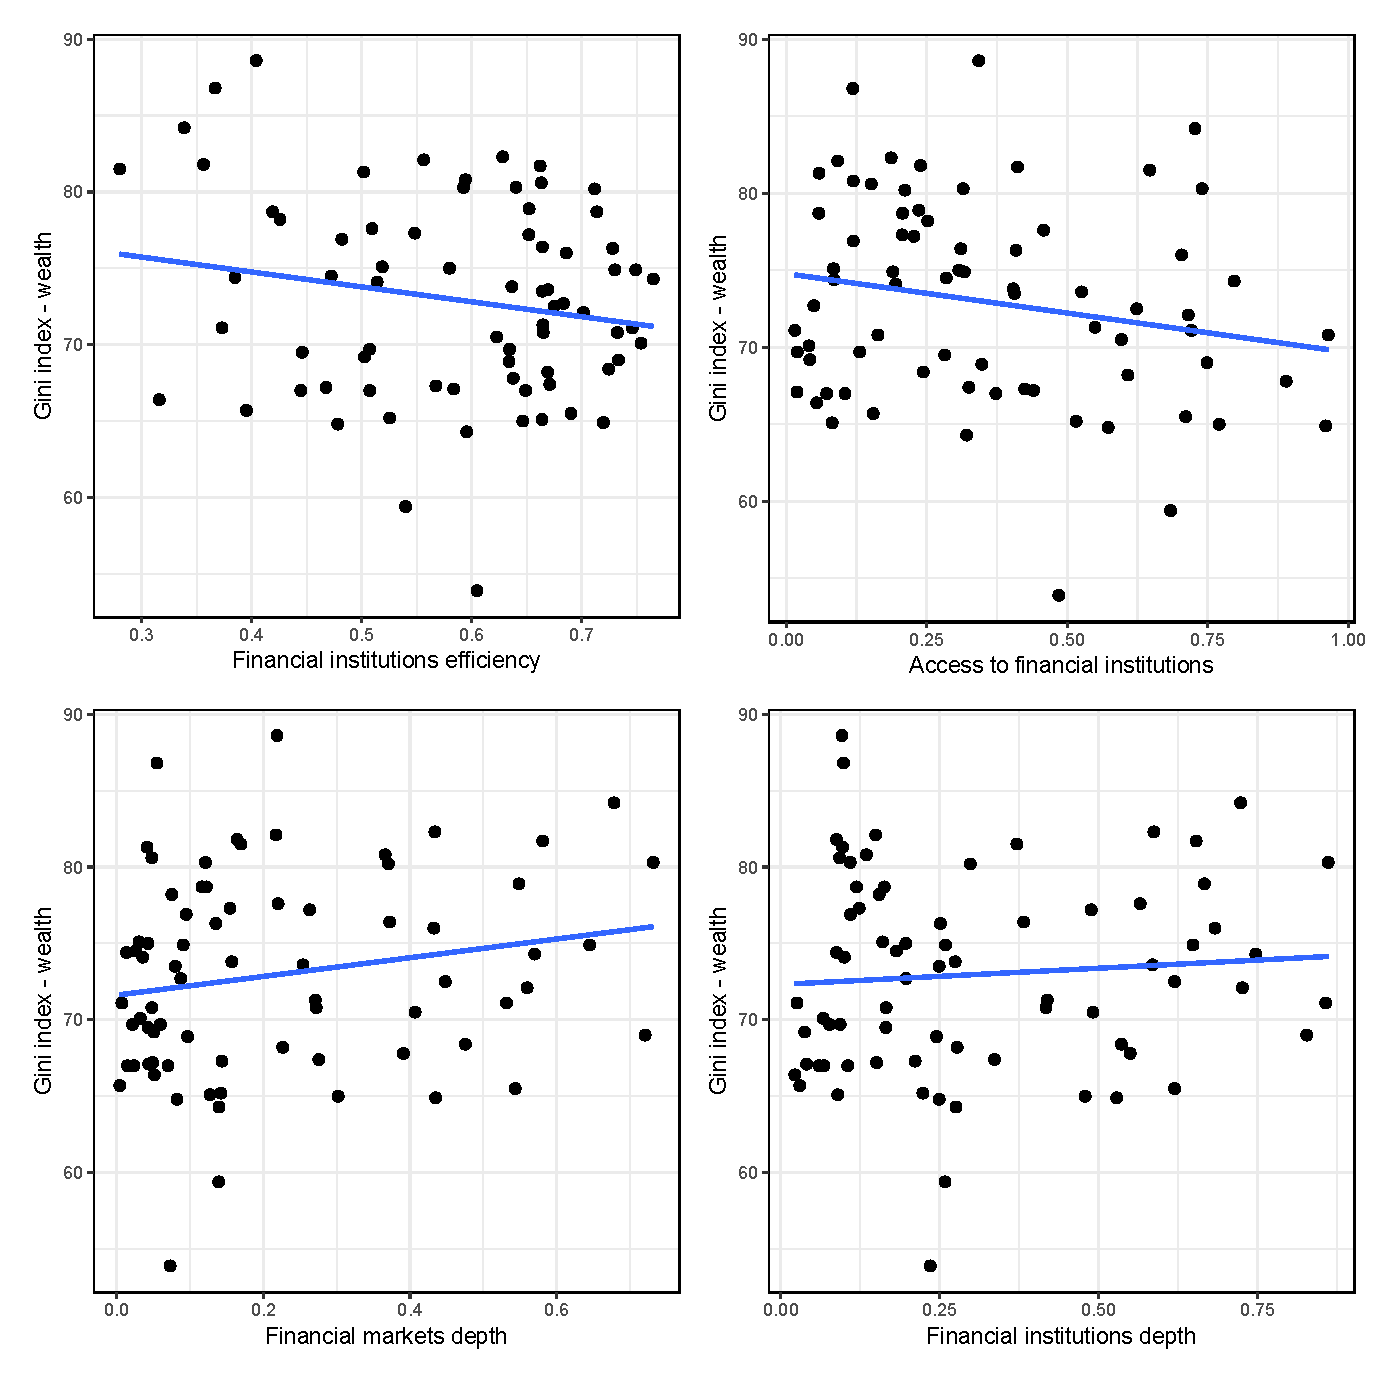
\includegraphics[width=0.85\textwidth, keepaspectratio]{figures/plots_findev.eps}
	\floatfoot*{\hspace{4em}Note: Selected financial development indicators.}
	\end{measuredfigure}
\end{figure}

% \begin{figure}[ht]
% \centering
% 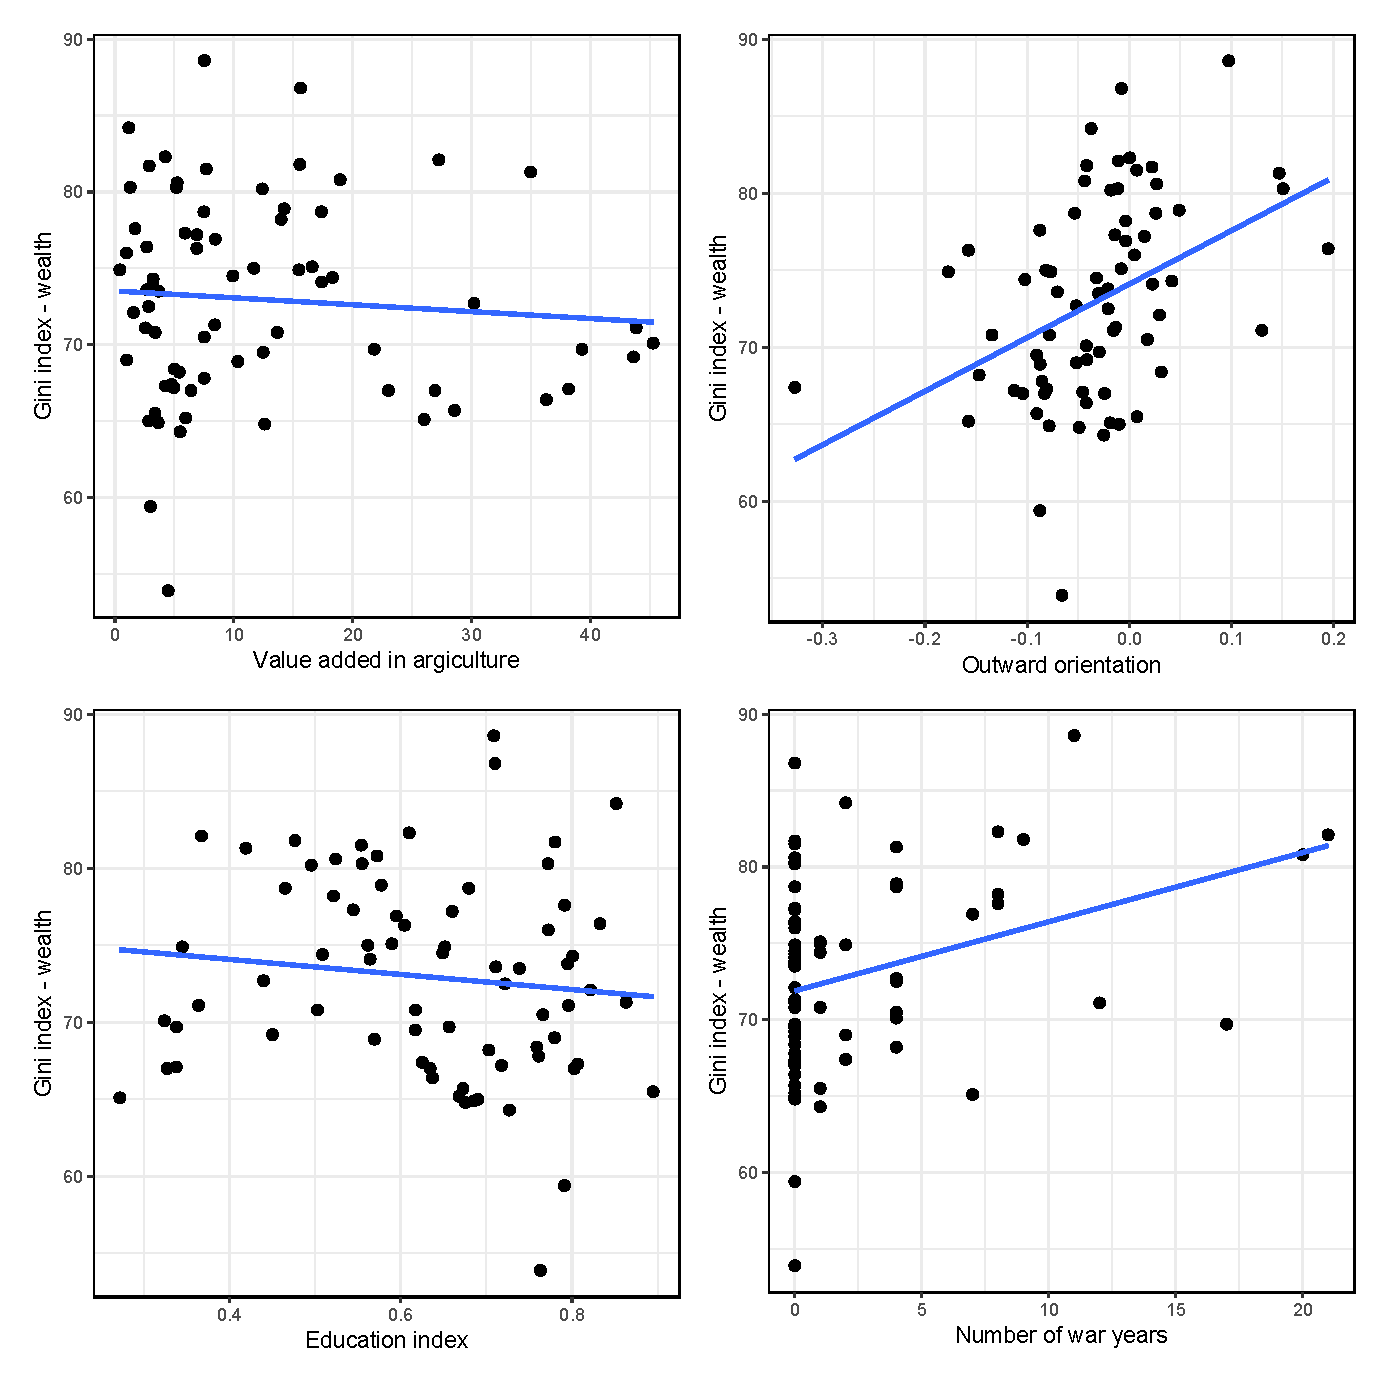
\includegraphics[width=0.85\textwidth, keepaspectratio]{figures/plots_highpips.eps}
% \caption{Wealth inequality and selected explanatory variables}
% \label{fig:highp}
% \end{figure}

Table \ref{table:res1} presents our BMA results regarding the determinants of wealth inequality. We present the explanatory variables sorted by their \ac{pip} values and interpret the results in accordance with \citet{kass1995bayes}, who present a conventional rule of thumb to evaluate the \ac{pip}. When the \ac{pip} is lower than 50\%, there is evidence against the effect, \ac{pip} between 50\% and 75\% suggest a weak evidence for the effect, \ac{pip} over 75\%, but less than 95\% means a “positive” evidence for the effect, in case of \ac{pip} higher than 95\%, but less than 99\% there is strong evidence for the effect, and \ac{pip} over 99\% provides decisive evidence for the effect.

According to our results, only a handful regressors robustly determines the cross-country variation in wealth inequality and exhibit \acp{pip} greater than 0.5. Financial development indicators represent nearly half of these regressors, suggesting that finance is a crucial factor for understanding wealth inequality. Examining our global sample, our results suggest that cross-country differences in wealth inequality are a combination of effects stemming from finance, globalization, education, advances in agriculture and redistribution. But quantitatively, how important is this set of regressors in explaining wealth inequality? If we estimate the simple OLS regression with regressors included in the model with the highest \ac{pmp}, we find the corresponding value of R-squared to be 0.57 (adjusted R-squared to be 0.52). This result suggests that we can explain approximately half of the variation in the cross-country differences in wealth inequality using only the eight most relevant regressors.\footnote{All regressors are statistically significant at the 1 or 10 percent level and exhibit signs of the coefficient estimates identical to those reported in Table \ref{table:res1}. Alternatively, we estimate the model by OLS using the regressors with \acp{pip} greater than 0.5 in the baseline \ac{bma}. The results again correspond to the \ac{bma} estimate. We report the output of both regressions in Table \ref{tab:ols} in the online Appendix.} We discuss the effects of individual regressors in detail below.

The variables with high \acp{pip} exhibit the expected qualitative effects on wealth distribution. The greater efficiency of financial intermediation and better access to the financial institutions results in a more uniform distribution of wealth. This finding is broadly in line with the conclusion of \citet{claessens2007finance} regarding the determinants of income inequality, who assert that access to financial resources is a key driver in reducing income inequality rather than the depth of the financial market. The result of \citet{claessens2007finance} also accords with the lower PIP of financial institutions depth in our model. 

According to our results, large financial markets (i.e., more capitalized stock markets and greater debt securities markets) propagate differences in wealth. Stock price booms are likely to increase wealth inequality because of the composition of household wealth, as stocks are typically owned by rich households. \citet{kuhn} provide new estimates of wealth inequality in the US from 1949--2016 based on archival data from the Survey of Consumer Finances and examine the evolution of wealth over time. Their results are in accordance with ours: stock price booms indeed contribute to greater wealth inequality.  

In addition, one could argue that our result regarding the effect of the size of financial markets on wealth inequality corresponds to recent findings suggesting that too much finance is harmful to growth \citep{Arcandetal2012,CecchettiKharroubi2012,LawSingh2014} and that it is important to disentangle quantity and quality of finance when examining the effect of finance on growth \citep{hasan2016}. However, this analogy is only partially valid because whereas we typically think of greater economic performance as a positive phenomenon, there is a uncertainty about what is the `optimal' level of wealth inequality. 

Outward orientation capturing the openness of the economy leads to higher levels of wealth inequality. Large importance and qualitative effect correspond to the earlier findings, such as those of \citet{dabla2015causes}, which claim that globalization and increasing exposure to the outside world contributes to greater within-country inequality. If globalization increases growth, then this result implies that the globalization benefits some economic agents more than others. For example, \citet{dabla2015causes} and \citet{milanovic2016global} mention the skill premium related to technological progress, which leads to excessive earnings and widens inequality. Nevertheless, our results provide little evidence that technological progress increases wealth inequality. We use a comprehensive index of technological progress developed by \citet{comin}, but as we can observe from Table \ref{table:res1}, its PIP is very low. We attribute our result regarding the effect of technological progress on wealth inequality to the sample that we use. Our global sample covers countries with different degrees of economic development and technological progress, and it is likely that technological progress may play a greater role specifically in the most advanced countries. 

Redistribution, which we define as the difference between the market and after-tax income Gini indexes, contributes to lower wealth inequality. This result can be interpreted as evidence indicating that government policies may in fact affect inequality despite the well-known difficulties regarding the taxation of top earners. Our results are broadly in line with those of \citet{jakobsen2018}, who find that the abolition of the Danish wealth tax in 1997 contributed to more wealth inequality by increasing the wealth of top earners. Interestingly, the political orientation of the government (as captured by the variable `left wing orientation') is not robustly related to wealth inequality. This result suggests that deeds (i.e., the actual level of redistribution) rather than words (i.e., stated political orientation) matter.\footnote{In one of the robustness checks, we also consider the relative redistribution (percentage reduction in market-income inequality due to taxes and transfers) Employing the alternative indicator of redistribution does not have any substantial impact on the other explanatory variables. The output of the estimation is available in Table \ref{table:relred} in the online Appendix.}.

Although the variable `number of war years' exhibits an inclusion probability of slightly less than 0.5, we find wars to be associated with higher wealth inequality. This result is at odds with previous evidence arguing that wars reduce inequality because of enormous capital destruction, inflation and sizable redistributive government programs (to finance the war); see, for example, \citep{piketty2014,milanovic2016global} and the references therein. However, this evidence focuses on the effect of war on inequality over time and focuses on substantial and long-lasting conflicts, such as World War I or II. Our regressions explain cross-sectional variation in wealth inequality, i.e., why inequality is higher in some countries than in others. In addition, our dataset regarding wars is based on the period after World War II, i.e., typically internal conflicts (civil wars) or conflicts involving a single or small number of countries. These conflicts have adverse macroeconomic effects, undermine the rule of law, cause violent confiscation of private property by militias and reduce trust in society, especially if these conflicts occur repeatedly \citep{bircanetal}. \citet{bircanetal} study the effect of internal violent conflicts on income inequality and also find inequality increases, but this effect is temporary, and later on, inequality falls slowly back to the steady state.

\begin{table}[!ht]
\footnotesize
\centering
\caption{Determinants of Wealth Inequality, BMA Estimation}
\label{table:res1}
\begin{threeparttable}
\begin{tabular}{lrrr}
  \toprule
 & PIP & Post Mean & Post SD \\ 
    \midrule
  Financial institutions efficiency & 1.00 & -0.33651 & 0.11350 \\ 
  Value added in agriculture & 1.00 & -0.51800 & 0.16188 \\ 
  Access to financial institutions & 1.00 & -0.38266 & 0.15020 \\ 
  Outward orientation & 0.87 & 0.20663 & 0.12371 \\ 
  Education index (UN) & 0.79 & -0.26055 & 0.20440 \\ 
  Financial market development & 0.77 & 0.34023 & 0.23533 \\ 
  Redistribution & 0.51 & -0.10670 & 0.13963 \\ 
  Number of war years & 0.48 & 0.06956 & 0.09701 \\ 
  Net national savings & 0.42 & 0.08447 & 0.13021 \\ 
  Economic freedom index (adjusted) & 0.35 & -0.08233 & 0.15183 \\ 
  Financial institutions development & 0.33 & 0.14210 & 0.24598 \\ 
  Natural resource rents & 0.29 & 0.04572 & 0.09402 \\ 
  Net foreign direct investment & 0.25 & -0.03291 & 0.07552 \\ 
  Average GDP growth & 0.22 & -0.02607 & 0.06759 \\ 
  Labor market regulation & 0.16 & 0.01630 & 0.05386 \\ 
  Leftwing orientation & 0.15 & -0.01239 & 0.04533 \\ 
  Population density & 0.14 & -0.01540 & 0.05521 \\ 
  Inflation & 0.12 & 0.01036 & 0.04442 \\ 
  Government expenditures & 0.12 & 0.01311 & 0.05717 \\ 
  Latin America dummy & 0.10 & 0.00987 & 0.04762 \\ 
  Financial markets efficiency & 0.09 & -0.00706 & 0.04026 \\ 
  Banking diversification & 0.09 & -0.00579 & 0.03217 \\ 
  Rule of law & 0.09 & 0.01368 & 0.08087 \\ 
  Active banking restrictions & 0.09 & -0.00612 & 0.03667 \\ 
  Financial development index (EFW) & 0.07 & -0.00364 & 0.04464 \\ 
  Public education expenditures & 0.07 & 0.00363 & 0.02903 \\ 
  Revolutions and coups & 0.07 & 0.00250 & 0.02705 \\ 
  Population growth & 0.07 & 0.00394 & 0.04154 \\ 
  Bank capital regulations & 0.07 & -0.00323 & 0.02589 \\ 
  GDP level in 1990 & 0.07 & -0.00809 & 0.07483 \\ 
  Civ. liberties and pol. rights & 0.06 & -0.00322 & 0.04104 \\ 
  Technological progress & 0.06 & -0.00596 & 0.06110 \\ 
  Life expectancy & 0.05 & 0.00043 & 0.04581 \\ 
  Financial openness (Chinn-Ito) & 0.05 & 0.00150 & 0.03218 \\ 
  Business conditions & 0.05 & -0.00196 & 0.02568 \\ 
  Value added in industry & 0.05 & -0.00030 & 0.02710 \\ 
  Labor force participation & 0.04 & 0.00054 & 0.01815 \\ 
  \midrule
  \bottomrule
\end{tabular}
\begin{tablenotes}
\item Note: Dependent variable - average Gini index (wealth) 2010-2016, 73 observations, baseline (hyper-g parameter prior) 
\end{tablenotes}
\end{threeparttable}
\end{table}

\clearpage
\begin{figure}
	\caption{Robustness Check: Different Prior Structure}
	\centering
	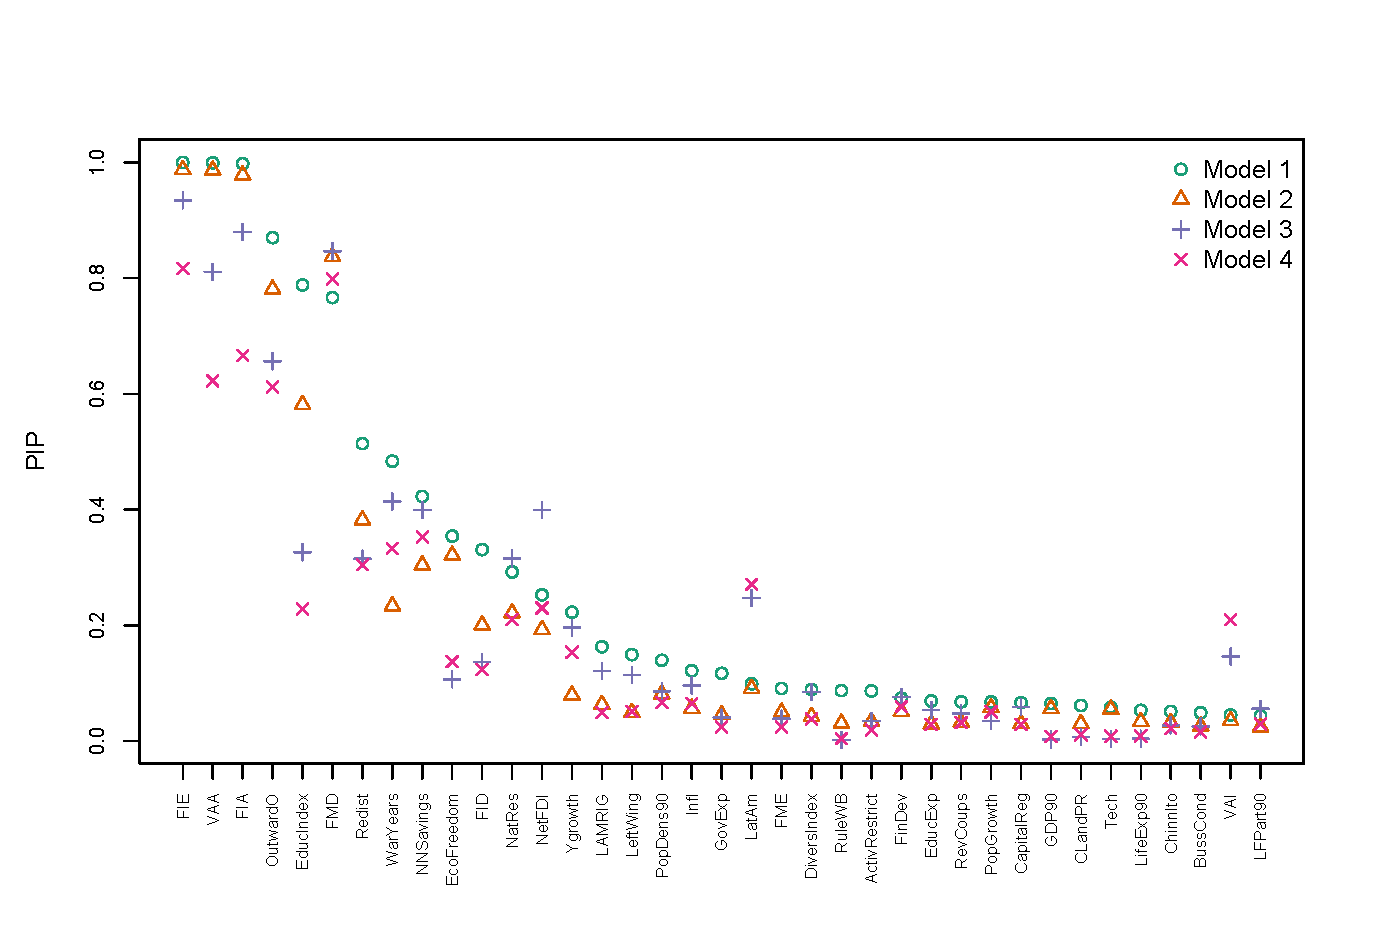
\includegraphics[width=0.9\textwidth]{figures/priors_comparison_compound.eps}
	\label{fig:comp_compound}
\floatfoot*{Note: Parameter and model prior comparison - compound indicators. Model 1: hyper-g, uniform; Model 2: UIP, uniform; Model 3: hyper-g, dilution; Model 4: UIP, dilution.}
\end{figure}

We report the baseline results, in which we employ the uniform model prior and hyper-g parameter prior, as described in section \ref{sec:BMA}. To provide robustness checks, we also use alternative parameter and model priors. Figure \ref{fig:comp_compound} presents a graphical illustration of our robustness checks. We estimate alternative specifications of the model using \ac{uip} and the dilution model prior described earlier. Overall, the results are similar. The optional priors slightly decrease \ac{pip} across the set of regressors, with the combined effect of \ac{uip} and dilution model prior having the largest effect. This slight overall decrease in inclusion probabilities is related to the smaller models dictated by the alternative prior structures, but the ordering of the variables in terms of \ac{pip} remains quite stable. The only exception to marginal decreases in the \ac{pip} is the effect of education, which decreases to less than 0.5 when we apply the dilution model prior in the estimation. This result could be partially explained by the design of this particular prior, which should down-weight variables that are highly correlated with others. We also tried other specifications with quadratic terms of financial indexes, interactions between the rule of law and financial indexes, and others.\footnote{For example, we investigate cases where we drop groups of variables as defined in Table \ref{tab:groups} in the online Appendix. Interestingly, when we drop a group of low \ac{pip} variables, the results are stable. On the other hand, if we drop a group which contains variables with high \ac{pip}s, the results deviate from the baseline estimates. This could be due to the introduction of omitted variable bias in the latter case as dropping important regressors may severely affect coefficients on the remaining variables.} None of these additional regressors exhibited significant relevance in our model.\footnote{These additional estimation results are available upon request.}

Next, we argue that the effect of finance on wealth inequality is complex and whereas some financial indicators decrease the inequality, other financial indicators increase it. But what is the overall effect of finance on wealth inequality? We take the estimated posterior means from Table \ref{table:res1} for the finance variables with PIP values greater than 0.5 (these are access to financial institutions (FIA), their efficiency (FIE), and the depth of stock market (FMD)) and multiply them by the corresponding country-specific values. Given the manner in which our explanatory variables are normalized, this multiplication is identical to examining the change in wealth inequality as a result of one-standard-deviation increases in FIA, FIE, and FMD. 

We present the results of overall effect of finance on wealth inequality in Figure \ref{fig:finance_effect}. Even though we do not want to overemphasize the precision of our results, the estimated effect is negative for all countries in our sample, i.e., our results suggest that greater financial development reduces wealth inequality. Nevertheless, we observe some heterogeneity in the estimated effect across the countries. Interestingly, we observe the weakest decreasing effect of finance on wealth inequality for the \ac{us}.\footnote{Alternatively, we assessed the overall effect of finance on wealth inequality based on the estimation of the ordinary least squares model. We selected the explanatory variables that had PIP values in Table \ref{table:res1} greater than 0.5. The results are largely the same and are available Table \ref{tab:ols} in the online Appendix.}

\begin{sidewaysfigure}
\begin{center}
\caption{Effects of individual financial development components on inequality}
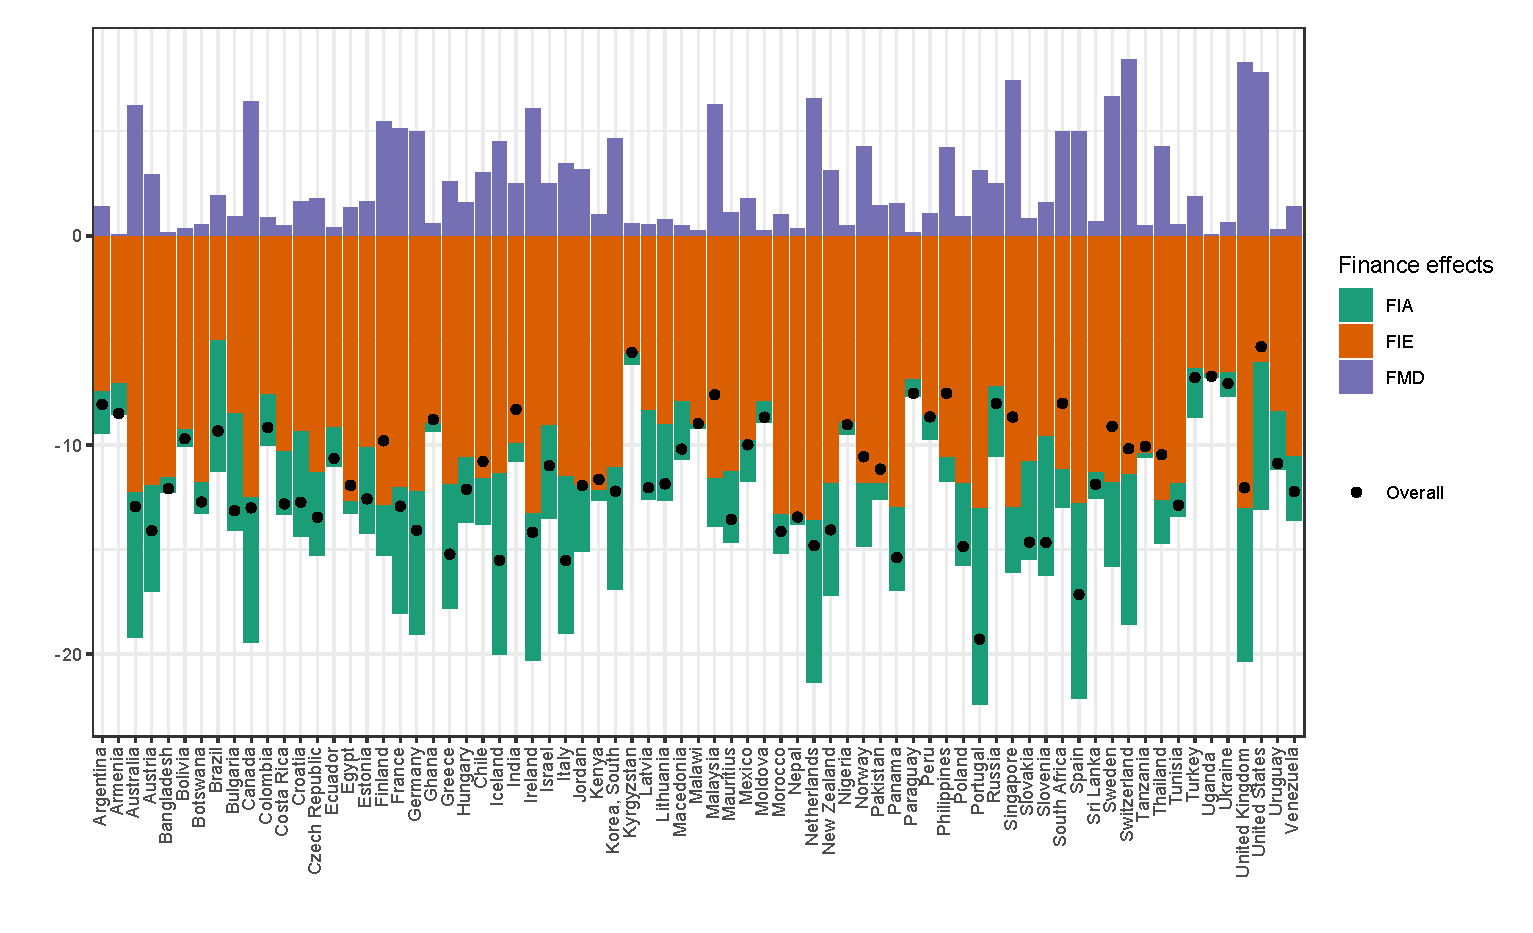
\includegraphics[width=0.95\textwidth]{figures/finance_effect.eps}
\label{fig:finance_effect}
\end{center}
\end{sidewaysfigure}

\subsection{High vs. low-income countries}
We explore the non-linearity of the estimated effects by splitting our sample into two halves according to the level of GDP in 1990. Such an exercise, however, presents an issue for the estimation with the full set of explanatory variables as only 36 observations remain in each sample. To overcome this, we consider nine explanatory variables which occur in the top three models by their \ac{pmp} which gives us enough degrees of freedom for the estimation. 

We present the results in Table \ref{tab:inc_comparison}. The estimated coefficients of explanatory variables have their expected signs. We observe some heterogeneity in terms of PIPs. We find that technological advancement in agriculture (value added in agriculture) and openness of the economy (outward orientation) are dominant factors for low-income countries, while they are less relevant for the group of high-income countries. This is expected result given the prominence of agriculture sector in developing countries. Wars matter both for low-income and high-income countries. Regarding the financial variables, depth of the financial market increases wealth inequality both in low-income and high-income countries. Other financial variables (access to finance and efficiency of financial intermediaries) reduce wealth inequality especially in high-income countries. This suggests that the role of finance for wealth inequality rises with economic development.  

\begin{table}[htbp!]
\caption{Estimates using the variables from the model with the highest posterior model probability and sample split into high- / low- income countries (based on GDP90)}
\label{tab:inc_comparison}
\centering
\begin{tabular}{lrrrr}
  \toprule
  & \multicolumn{2}{c}{High-income} & \multicolumn{2}{c}{Low-income} \\
  \midrule
	 & PIP & Post. Mean & PIP & Post. Mean \\ 
  \midrule
  Financial market depth & 0.97 & 0.55171 & 0.66 & 0.21279 \\ 
  Average GDP growth & 0.83 & -0.31499 & 0.23 & 0.00877 \\ 
  Access to financial institutions & 0.76 & -0.30279 & 0.27 & 0.04851 \\ 
  Number of war years & 0.72 & 0.36526 & 0.62 & 0.09226 \\ 
  Financial institutions efficiency & 0.60 & -0.22569 & 0.24 & -0.00668 \\ 
  Redistribution & 0.56 & -0.16593 & 0.27 & -0.02704 \\ 
  Outward orientation & 0.50 & 0.11034 & 1.00 & 0.36512 \\ 
  Education index (UN) & 0.38 & -0.10648 & 0.32 & -0.04479 \\ 
  Value added in agriculture & 0.29 & 0.03537 & 0.94 & -0.33730 \\ 
   \bottomrule
\end{tabular}
\end{table}

% \begin{figure}[ht!]
% 	\caption{PIP comparison using the variables from the model with highest posterior model probability and sample split into high- / low-income countries (based on GDP90)}
% 	\centering
% 	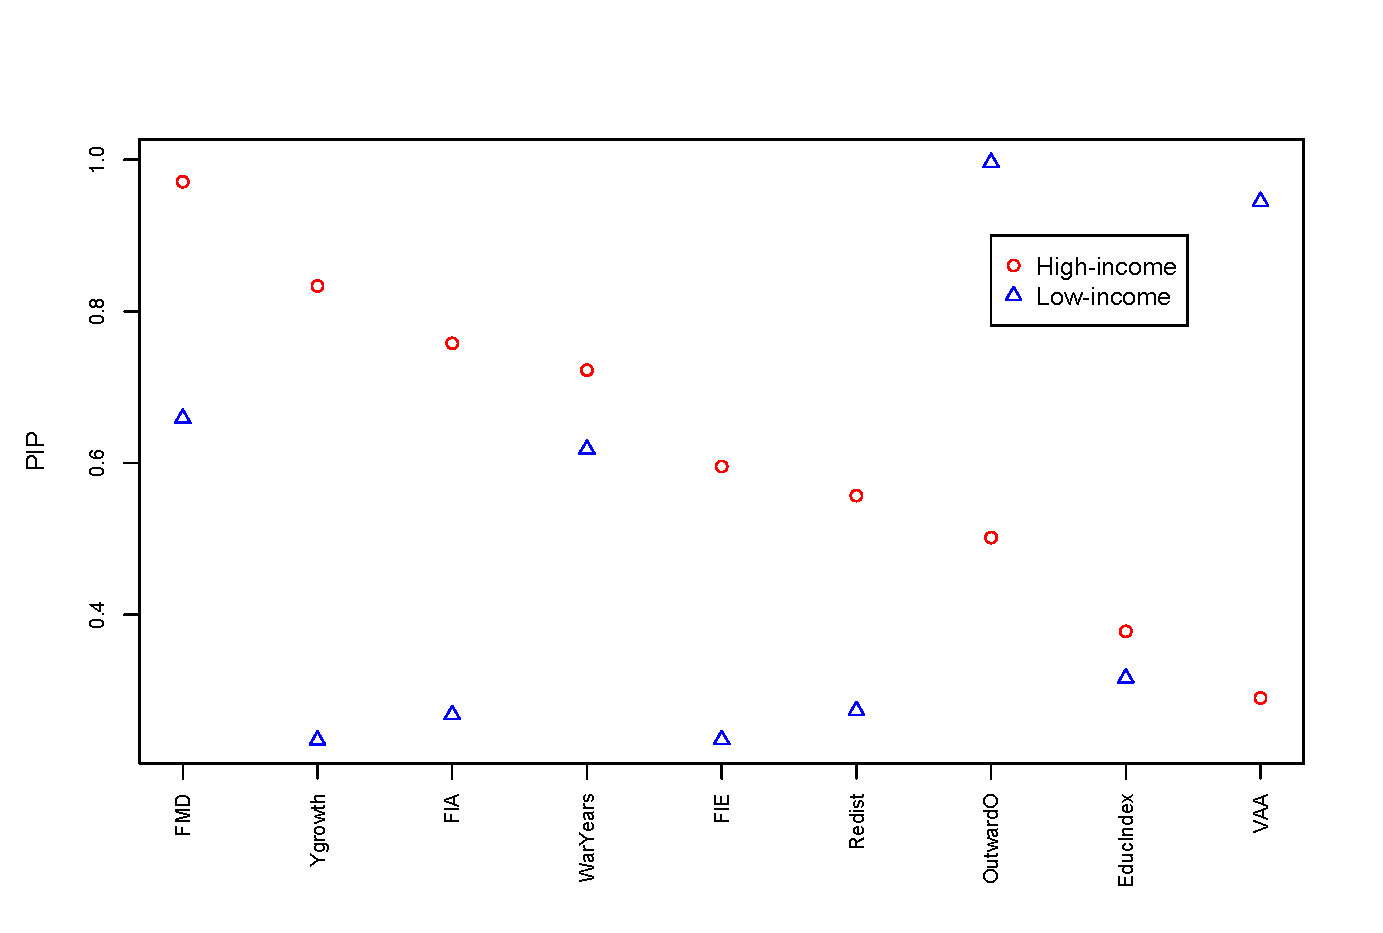
\includegraphics[width=0.9\textwidth]{figures/low_high_inc_comparison.eps}
% 	\label{fig:inc_comparison}

% 	Source: Authors'
% \end{figure}

% \begin{table}[htbp!]
% \caption{Estimates using the variables from the model with highest posterior model probability and restricted sample of low-income countries (based on GDP90)}
% \label{tab:l_inc}
% \centering
% \begin{tabular}{lrrr}
%   \hline
% 	 & PIP & Post Mean & Post SD \\ 
%   \hline
%   Outward orientation & 1.00 & 0.36512 & 0.09174 \\ 
%   Value added in agriculture & 0.94 & -0.33730 & 0.14182 \\ 
%   Financial market depth & 0.66 & 0.21279 & 0.20351 \\ 
%   Number of war years & 0.62 & 0.09226 & 0.09600 \\ 
%   Education index (UN) & 0.32 & -0.04479 & 0.10874 \\ 
%   Redistribution & 0.27 & -0.02704 & 0.08046 \\ 
%   Access to financial institutions & 0.27 & 0.04851 & 0.16716 \\ 
%   Financial institutions efficiency & 0.24 & -0.00668 & 0.05339 \\ 
%   Average GDP growth & 0.23 & 0.00877 & 0.04433 \\ 
%    \hline
% \end{tabular}
% \end{table}
\clearpage

\subsection{Endogeneity issues}
In our baseline results, we address endogeneity issues by estimating the effect of lagged regressors on wealth inequality. While wealth inequality is based on the data between 2010-2016, the regressors are based on data prior 2010 and often cover the 1980s, 1990s or 2000s. Therefore, we followed the procedure typical for BMA literature \citep{christofides,feldkircherjimf,hasan2016}.  

The question of endogeneity is, however, deeply ingrained in the finance-inequality nexus, and we want to provide additional evidence that the estimated effect of finance on wealth distribution is causal. There are reasons for caution. First, a wealth distribution that is more concentrated at the top may result in more power of incumbents, who lobby for funding of their projects using their political connections and thereby distort the market. Second, making the distribution of wealth more equal may lead to increased demand for financial services as more individuals seek to invest their savings or take up loans when their wealth provides a satisfactory collateral. If such development leads to increased supply of financial services through, for example, newly installed ATMs and opened institutions, it may manifest as better access to financial services \citep{beck2007finance}.

To address the potential endogeneity of the relationship between wealth distribution and financial development, we apply \ac{ivbma}. This methodology suggested by \cite{KarlLenkoski2012} implements the idea of instrumental variables in a Bayesian framework. It is essentially a two-stage estimation in which model uncertainty is considered in both stages. In the robustness check, we set the depth of financial institutions and access to financial institutions endogenous, as we believe that from our set of financial indicators, these are most the ones most likely affected by the reverse causality issues presented previously.

We employ genetic distance from the United States \citep{spolaore2009diffusion} along with a measure of financial liberalization as instruments. The financial liberalization proxy we construct relies on the components of \ac{efw} index by \citep{gwartney2017}. More specifically, we average the areas 3D, 4C, 4D, and 5A of the \ac{efw}. These represent freedom to own foreign currency accounts, black-market exchange rate premium, controls on the movement of capital and people, and credit market regulations. We refer to the authors of \ac{efw} for the details of individual components. Although the search for good instruments is a nontrivial exercise, we believe our choice satisfies the basic conditions. Genetic distance should be unrelated to wealth distribution\footnote{In our sample, the correlation is 0.06.}. Even if the primary cause of migration is more/less equal distribution of wealth, it would most likely not be sufficiently substantial to affect the genetic pattern in a particular country. Additionally, the components of our financial liberalization measure are exogenous to the wealth inequality as the change in wealth distribution is improbably to have direct effect on any of them. We follow \citet{estev} here, who treat foreign trade liberalization as exogenous.

We check the strength of our instruments by examining the correlations and running simple OLS regressions of our endogenous variable on the instruments. The correlations of the instruments are greater than 0.5 in absolute terms, with the only exception being FID and genetic distance, for which it is -0.37. The regressions reveal strong significance of the instruments and the F-test statistics of the regressions are 35.43 and 19.95 for FIA and FID, respectively. Both values are well above 10, the rule of thumb proposed by \citet{staiger1997instrumental}. We have compared several additional instruments often used in the literature, including the ubiquitously used financial reform index by \citet{Abiadetal2008} and the legal origin of the countries, but the \ac{efw} measure turned out to be the strongest of the instruments. Our main \ac{ivbma} results rely on the just-identified case where we have two potential instruments for two potentially endogenous variables. We check the overidentification with Sargan test as introduced in \citet{lenkoski2014two}, where the Sargan p-value is an weighted average of p-values from individual combinations of first and second stage models weighted by their model probabilities. The values are only available for potentially overidentified cases, where the number of instruments considered in the first stage is higher than the number of assumed endogenous variables. The averaged p-value from these cases confirms the validity of instruments.

Table \ref{table:res_endo} presents the results of the \ac{ivbma} estimation. The \acp{pip} of instrumented variables somewhat decrease, in the case of access to financial institutions slightly below 0.5, but it still remains among the most important regressors. We also confirm the positive effect of financial markets depth along with the high inclusion probability. The \acp{pip} cannot be directly compared with the baseline results due to differences in the estimation procedure. Whereas for the standard \ac{bma} we report the inclusion probabilities based on the analytical posterior probabilities of the top models, \ac{ivbma} reports the probabilities based on the sampler. The latter approach tends to downweight the \ac{pip} for the top and upweight it for the bottom regressors.\footnote{If we compare \ac{ivbma} output with the MC3 \acp{pip} from the baseline \ac{bma}, we obtain very similar values for both approaches.} Overall, the \ac{ivbma} estimation largely supports our baseline findings. 

\begin{table}[!ht]
	\footnotesize
	\centering
	\caption{Determinants of Wealth Inequality, IVBMA Estimation}
	\label{table:res_endo}
	\begin{threeparttable}
	\begin{tabular}{lrrr}
		\toprule
		& PIP & Post. Mean & Post. SD\\ 
		\midrule
		Financial institutions efficiency & 0.85826 & -0.32431 & 0.18276 \\ 
		Value added in agriculture & 0.78741 & -0.39918 & 0.27546 \\ 
		Financial market depth & 0.62200 & 0.29196 & 0.32026 \\ 
		Financial institutions depth & 0.55682 & 0.24718 & 0.39989 \\ 
		Outward orientation & 0.52022 & 0.13647 & 0.15901 \\ 
		Economic freedom index (adjusted) & 0.50242 & -0.18778 & 0.24043 \\ 
		Education index (UN) & 0.46915 & -0.16719 & 0.23034 \\ 
		Access to financial institutions & 0.45168 & -0.19051 & 0.31849 \\ 
		Net national savings & 0.42093 & 0.11213 & 0.16687 \\ 
		Redistribution & 0.39198 & -0.10184 & 0.15932 \\ 
		Natural resource rents & 0.36756 & 0.08280 & 0.13856 \\ 
		Number of war years & 0.36660 & 0.07267 & 0.11648 \\ 
		GDP level in 1990 & 0.29348 & -0.03476 & 0.21811 \\ 
		Latin America dummy & 0.25851 & 0.05039 & 0.11744 \\ 
		Net foreign direct investment & 0.24740 & -0.04159 & 0.09389 \\ 
		Technological progress & 0.24198 & -0.02756 & 0.15284 \\ 
		Rule of law & 0.22111 & 0.00025 & 0.13277 \\ 
		Life expectancy & 0.21608 & -0.02082 & 0.12509 \\ 
		Value added in industry & 0.20523 & 0.03081 & 0.09693 \\ 
		Civ. liberties and pol. rights & 0.17607 & 0.00152 & 0.08731 \\ 
		Population growth & 0.17297 & 0.01557 & 0.08178 \\ 
		Inflation & 0.17219 & 0.02180 & 0.07214 \\ 
		Average GDP growth & 0.16884 & -0.01947 & 0.06804 \\ 
		Population density & 0.15698 & -0.01672 & 0.06680 \\ 
		Government expenditures & 0.15095 & 0.01087 & 0.06574 \\ 
		Labor market regulation & 0.14337 & 0.01307 & 0.05424 \\ 
		Financial openness (Chinn-Ito) & 0.13893 & -0.00881 & 0.06817 \\ 
		Leftwing orientation & 0.13809 & -0.01337 & 0.04972 \\ 
		Business conditions & 0.12686 & -0.00665 & 0.05531 \\ 
		Financial markets efficiency & 0.12605 & -0.00358 & 0.05153 \\ 
		Revolutions and coups & 0.12206 & 0.00728 & 0.04631 \\ 
		Active banking restrictions & 0.11903 & -0.00620 & 0.04858 \\ 
		Banking diversification & 0.11722 & -0.00860 & 0.04230 \\ 
		Public education expenditures & 0.10759 & 0.00368 & 0.03795 \\ 
		Bank capital regulations & 0.09251 & -0.00155 & 0.03023 \\ 
		Labor force participation & 0.09011 & -0.00148 & 0.02810 \\ 
		\bottomrule
	\end{tabular}
\begin{tablenotes}
\item Note: Dependent variable - average Gini index (wealth) 2010-2016, 73 observations. Financial depth of and access to financial institutions as endogenous. Instruments: genetic distance, financial development index from Economic Freedom of the World.
\end{tablenotes}
\end{threeparttable}
\end{table}

\section{Concluding Remarks}
\label{sec:conclusion}

This paper makes a new contribution to the burgeoning literature about wealth inequality. Whereas the existing literature focuses largely on measurement of wealth inequality \citep{alvaredoetal2013,daviesetal2011,pikettyandzucman2014,SaezZucman2016}, we examine a wide array of possible determinants of wealth inequality. 

Building the large cross-country dataset, we employ \ac{bma} to study the determinants of wealth inequality in order to address the regression model uncertainty. This uncertainty arises from the lack of an encompassing model of wealth inequality, which would dictate the exact regression specification to be estimated. As a side effect, using \ac{bma}, we can examine a large number of possible determinants of wealth inequality within a unifying framework. Therefore, we examine how different economic, financial, regulatory, political, social, and institutional variables affect wealth inequality.  

Using our global sample, addressing endogeneity issues and subjecting our results to a number of robustness checks, we find that only a handful variables are robustly related to wealth inequality. Our results suggest that cross-country differences in wealth inequality arise due to a combination of the effects stemming from the financial sector, globalization, education, advances in agriculture and government redistribution. More specifically, our baseline estimation shows that there are seven regressors with PIP values greater than 50\%, and they explain approximately half of the cross-country differences in wealth inequality. 

We find that finance plays an important role in wealth inequality. Out of seven aforementioned variables that are robustly related to wealth inequality, three of them capture the level of financial development. According to our results, finance exerts a complex effect on wealth inequality. Some financial characteristics increase inequality, whereas other financial characteristics, to the contrary, decrease it.

Our results show that large financial markets (as proxied by the stock market capitalization and size of debt securities market type of variables) are associated with greater wealth inequality. This result follows from the composition effect, as it is typically rich households that participate in the stock markets \citep{kuhn}. On the other hand, our findings show that countries with better access to finance and more efficient financial intermediaries exhibit lower wealth inequality. Therefore, there is no natural tendency that financial development results into greater wealth inequality. On the contrary, when we take the average values of financial development measures, the overall effect of finance development on wealth inequality is negative (i.e., more financially developed countries associated with lower level of wealth inequality). 

In addition, our results show that more education and greater income redistribution are associated with lower level of wealth inequality. Therefore, this result broadly suggest that governments can affect the inequality within their countries (either via education or taxation). In addition, we also find that (the lack of) political stability influences wealth inequality, as our results show that countries with war experience exhibit greater inequality. Finally, our results suggest that globalization but not technological development is likely to contribute to greater wealth inequality.

\clearpage
%
\bibliographystyle{chicagoa}
\bibliography{literature}
%
\clearpage
%
\appendix

\section*{Appendix}
\label{sec:app}

\renewcommand{\thesection}{A\arabic{section}}%
\renewcommand{\thetable}{A\arabic{table}}%
\renewcommand{\thefigure}{A\arabic{figure}}%
\renewcommand{\theequation}{A\arabic{equation}}%
\setcounter{equation}{0}%
\setcounter{table}{0}%
\setcounter{figure}{0}%

\subsection*{Dataset description}
\begin{center}
	\footnotesize
	\begin{longtable}{l p{0.50\linewidth} p{0.3\linewidth}}
		\caption{List of variables} 
		\label{app:data}
		\\
		\toprule
		Variable & Definition (+ optional comments) & Source \\
		\midrule
		GiniWealth & Gini index based on the distribution of wealth from Credit Suisse Wealth Reports 2010-2016 & \href{https://www.credit-suisse.com/cz/en/about-us/research/research-institute/global-wealth-report.html?WT.i_short-url=%2Fgwr&WT.i_target-url=%2Fcz%2Fen%2Fabout-us%2Fresearch%2Fresearch-institute%2Fglobal-wealth-report.html}{Credit Suisse} \\
			
			FIA & Access to financial institutions & \href{http://data.imf.org/?sk=F8032E80-B36C-43B1-AC26-493C5B1CD33B}{\citet{svirydzenka2016introducing}} \\
			
			FID & Financial institutions depth & \href{http://data.imf.org/?sk=F8032E80-B36C-43B1-AC26-493C5B1CD33B}{\citet{svirydzenka2016introducing}} \\
			
			FIE & Financial institutions efficiency & \href{http://data.imf.org/?sk=F8032E80-B36C-43B1-AC26-493C5B1CD33B}{\citet{svirydzenka2016introducing}} \\
			
			FMD & Financial markets depth & \href{http://data.imf.org/?sk=F8032E80-B36C-43B1-AC26-493C5B1CD33B}{\citet{svirydzenka2016introducing}} \\
			
			FME & Financial markets efficiency & \href{http://data.imf.org/?sk=F8032E80-B36C-43B1-AC26-493C5B1CD33B}{\citet{svirydzenka2016introducing}} \\
			
			GDP90 & Level of GDP per capita in 1990 & \href{http://febpwt.webhosting.rug.nl/Home}{PWT (9.0)} \\
			
			NatRes & Total natural resource rents are the sum of oil rents, natural gas rents, coal rents (hard and soft), mineral rents, and forest rents. Average 1980-2009 & \href{http://data.worldbank.org/indicator/NY.GDP.TOTL.RT.ZS}{WB} \\
			
			PopGrowth & Annual population growth 1980-2009 & \href{http://data.worldbank.org/indicator/SP.POP.GROW}{WB} \\
			
			GovExp & General government final consumption expenditure (formerly general government consumption). Average 1980-2009 & \href{http://data.worldbank.org/indicator/NE.CON.GOVT.ZS}{WB}\\
			
			NNSavings & Net national savings (gross national savings less the value of consumption of fixed capital, \% GNI). Average 1980-2009 & \href{http://data.worldbank.org/indicator/NY.ADJ.NNAT.GN.ZS}{WB} \\
			
			EducExp & Education expenditure refers to the current operating expenditures in education, including wages and salaries and excluding capital investments in buildings and equipment. Average 1980-2009. & \href{http://data.worldbank.org/indicator/NY.ADJ.AEDU.GN.ZS}{WB} \\
			
			Infl & Inflation as measured by the consumer price index. Average 1980-2009. & \href{http://data.worldbank.org/indicator/FP.CPI.TOTL.ZG}{WB} \\
			
			VAA & Agriculture, forestry, and fishing value added (\% GDP). Average 1980-2009. & \href{http://data.worldbank.org/indicator/NV.AGR.TOTL.ZS}{WB} \\
			
			VAI & Industry value added (\% GDP). Average 1980-2009. & \href{http://data.worldbank.org/indicator/NV.IND.TOTL.ZS}{WB} \\
			
			StartBussC & Cost of business start-up procedures (\% of GNI per capita). Average 1980-2009 & \href{http://data.worldbank.org/indicator/IC.REG.COST.PC.ZS}{WB} \\
			
			StartBussT & Time required to start a business (days). Average 1980-2009 & \href{http://data.worldbank.org/indicator/IC.REG.DURS}{WB} \\
			
			GFCF & Gross fixed capital formation (\% of GDP). Average 1980-2009 & \href{http://data.worldbank.org/indicator/NE.GDI.FTOT.ZS}{WB} \\
			
			NetFDI &  Foreign direct investment, net inflows (\% of GDP). Average 1980-2009 & \href{http://data.worldbank.org/indicator/BX.KLT.DINV.WD.GD.ZS}{WB} \\
			
			Ygrowth & Annual growth of GDP. Average 1980-2009 & \href{http://www.rug.nl/research/ggdc/data/pwt/pwt-9.0}{PWT 9.0} \\
			
			LifeExp90 & Life expectancy at birth in 1990 & \href{http://data.worldbank.org/indicator/SP.DYN.LE00.IN}{WB}\\
			
			LabForce90 & Total labor force comprises people ages 15 and older who meet the International Labor Organization definition of the economically active population: all people who supply labor for the production of goods and services during a specified period. Labor force total, 1990. Not available before 1990. & \href{http://data.worldbank.org/indicator/SL.TLF.CACT.ZS}{WB} \\
			
			PopDens90 & Population density (people per sq. km of land area) in 1990. & \href{http://data.worldbank.org/indicator/EN.POP.DNST}{WB} \\
			
			RevCoups & Revolutions and coups, total instances between 1950 and 2010 & \href{http://jpr.sagepub.com/content/48/2/249.abstract}{Powell and Thyne (2011)} \\
			
			EthnoLfrac & Ethnolinguistic franctionalization. The most detailed/disaggregated fractionalization measure (ELF.15 in the original paper) is assumed as it is found most relevant to growth and has highest correlation with other fractionalization measure by \href{http://www.nsd.uib.no/macrodataguide/set.html?id=16&sub=1}{Alesina et al. (2003)} & \href{http://www.anderson.ucla.edu/faculty_pages/romain.wacziarg/papersum.html}{Desmet et al. (2009)} \\
			
			WarYears & Number of war years (including civil wars) between 1946-2009 as defined in the UCDP dataset (more than 1000 casulties within a year) & \href{http://www.pcr.uu.se/research/ucdp/datasets/ucdp_prio_armed_conflict_dataset/}{UCDP/PRIO data} \\
			
			RuleOfLaw & Rule of law 1970-2009 (\textit{alternatively WB has data 1996-2014})& \href{http://efwdata.com/grid/WxRvYnU#/Grid}{Fraser institute} \\
			
			CivLib & Civil liberties 1973-2009 & \href{https://freedomhouse.org/report/freedom-world-2016/methodology}{Freedom House} \\
			
			PolRights & Political rights 1973-2009 & \href{https://freedomhouse.org/report/freedom-world-2016/methodology}{Freedom House} \\
			
			OutwardO & Measure of outward orientation derived as Net exports/GDP (\textit{previously based on data 1950-1983}) & \href{http://www.rug.nl/research/ggdc/data/pwt/pwt-9.0}{PWT 9.0} \\
			
			LatAm & 1 for Latin American countries & \\
			
			ChinnIto & Chinn-Ito index of financial opennes. Average 1980-2010. & \href{http://web.pdx.edu/~ito/Chinn-Ito_website.htm}{Chinn-Ito} \\ 
			
			LeftWing & Number of years between 1980 and 2009 when left oriented party lead the country. & \href{http://www.nsd.uib.no/macrodataguide/set.html?id=11&sub=1}{DPI} \\
			
			ActivRestrict & Activity restrictions. Regulatory restrictions on bank activities and the mixing of banking and commerce. & \href{http://faculty.haas.berkeley.edu/ross_levine/regulation.htm}{Barth et al. (2013)} \\
			
			CapitalReg & Capital Regulatory index. & \href{http://faculty.haas.berkeley.edu/ross_levine/regulation.htm}{Barth et al. (2013)} \\
			
			DiversIndex & Whether there are explicit, verifiable, quantifiable guidelines for asset diversification and banks are allowed to make loans abroad. & \href{http://faculty.haas.berkeley.edu/ross_levine/regulation.htm}{Barth et al. (2013)} \\
			
			LAMRIG & Index capturing the rigidity of employment protection legislation & \href{https://www.iza.org/publications/dp/6881}{Campos \& Nugent (2012)} \\
			
			Tech & Index on the level of technological development based on CHAT dataset & \href{http://www.nber.org/data/chat/}{Comin \& Hobijn (2009)} \\
			
			EducIndex & Calculated using mean years of schooling and expected years of schooling & \href{http://hdr.undp.org/en/content/education-index}{UN} \\
			
			NetInterestMargin & Accounting value of banks' net interest revenue as a share of average interest-bearing assets; a measure of the efficiency of the banking sector. & \href{http://data.worldbank.org/data-catalog/global-financial-development}{GFDD} \\
			
			BankZScore & return on banks' assets plus the ratio of banks' equity and assets, divided
			by the standard deviation of the return on assets (ROA+equity/assets)/sd(ROA); a measure of stability of the banking sector & \href{http://data.worldbank.org/data-catalog/global-financial-development}{GFDD} \\
			
			Privatecredit & Domestic private credit to the real sector to GDP; a measure of the depth of the banking sector & \href{http://data.worldbank.org/data-catalog/global-financial-development}{GFDD} \\
			
			MarketCap & Value of listed shares to GDP; a measure of the
			depth of stock markets.& \href{http://data.worldbank.org/data-catalog/global-financial-development}{GFDD} \\
			
			MarketTurn & Stock market value traded to total market capitalization; a measure of the efficiency of stock markets. & \href{http://data.worldbank.org/data-catalog/global-financial-development}{GFDD} \\
			
			BankBranches & Number of bank branches per 100,000 adults & \href{http://data.worldbank.org/data-catalog/global-financial-development}{GFDD} \\
			
			Loan2Deposits & Loan-to-deposit ratio. & \href{http://data.worldbank.org/data-catalog/global-financial-development}{GFDD} \\
			
			Redist & Difference between market (pre-tax) and net (after-tax0 Gini index based on distribution of income  (The Standardized World Income Inequality Database). & \href{http://fsolt.org/swiid/}{Solt (2016)} \\	
			
			FST & Genetic distance data (distance from the US) & \href{https://sites.tufts.edu/enricospolaore/research/}{\citet{spolaore2009diffusion}} \\
			
			FinReform & Financial reform index by Abiad (2010) & \href{https://www.imf.org/en/Publications/WP/Issues/2016/12/31/A-New-Database-of-Financial-Reforms-22485}{\citet{Abiadetal2008}} \\
			
			FinLib & Averaged components of Economic Freedom of the World index 3D (freedom to own foreign currency accounts), 4C (black-market exchange rates), 4D (controls of the movement of capital and people), and 5A (credit market regulations). & \href{https://www.fraserinstitute.org/economic-freedom/dataset}{\citet{gwartney2017}} \\
			
		\end{longtable}
	\end{center}


\end{document}